% Copyright 2007 by Till Tantau
%
% This file may be distributed and/or modified
%
% 1. under the LaTeX Project Public License and/or
% 2. under the GNU Public License.
%
% See the file doc/licenses/LICENSE for more details.


\documentclass{beamer}

% Setup appearance:

\usetheme{PaloAlto}
\usefonttheme{structurebold}
%\usecolortheme{crane}
\definecolor{mygold}{RGB}{255,204,0}
\definecolor{chocolate}{RGB}{97,51,24}
\definecolor{mygreen}{RGB}{173,214,50}
\setbeamercolor{structure}{bg=chocolate, fg=white}
\setbeamercolor{palette primary}{use=structure,fg=mygold,bg=chocolate}
\setbeamercolor{sidebar}{bg=chocolate,fg=white}
\setbeamercolor{sidebar}{parent=palette primary}
\setbeamercolor{section in sidebar shaded}{fg= mygold}
\setbeamercolor{subsection in sidebar shaded}{fg= mygreen}
\setbeamercolor{item projected}{fg=white,bg=chocolate}
\setbeamercolor{block body alerted}{bg=normal text.bg!90!chocolate}
\setbeamercolor{block body}{bg=normal text.bg!90!chocolate}
\setbeamercolor{block body example}{bg=normal text.bg!90!chocolate}
\setbeamercolor{block title alerted}{use={normal text,alerted text},fg=alerted text.fg!75!normal text.fg,bg=normal text.bg!75!chocolate}
\setbeamercolor{block title}{bg=chocolate}
\setbeamercolor{block title example}{use={normal text,example text},fg=example text.fg!75!normal text.fg,bg=normal text.bg!75!chocolate}

\addtobeamertemplate{footline}
{%
   \usebeamercolor[fg]{author in sidebar}
   \vskip-1cm\hskip10pt
   %\insertpagenumber\,/\,\insertpresentationendpage\kern1em\vskip2pt%
   \insertframenumber\,/\,\inserttotalframenumber\kern1em\vskip2pt%
}


\setbeamerfont{frametitle}{size=\normalsize,series=\bfseries}
\setbeamertemplate{navigation symbols}{}

% Standard packages

\usepackage{amsmath,amsthm,amssymb,latexsym,hyperref,url,graphicx,multicol}
\usepackage{color}
\usepackage{setspace,tikz,scalefnt}
\usepackage{multirow}
\usepackage{caption}
\usepackage{hyperref}

\graphicspath{ {./Figures/} }

\logo{
\includegraphics[scale=.3]{shield5}}

% The main document
%\setbeamercovered{transparent}

\usepackage{graphicx} % Allows including images
\usepackage{caption}
\usepackage{subcaption}
\usepackage{verbatim}
\usepackage{xcolor}
\hypersetup{
	colorlinks=true,
	linkcolor=blue,
	filecolor=magenta,      
	urlcolor=cyan,
}

%----------------------------------------------------------------------------------------
%	TITLE PAGE
%----------------------------------------------------------------------------------------

\title[Call Center Analysis]{Analysis, Visualization, and Simulation of Call Center Data} % The short title appears at the bottom of every slide, the full title is only on the title page

%* to show who is speaking
\author[Bulger \and Schmitt]{Presented by John D. Bulger\\ Graduate Student, Analytics \& Modeling
\\ \vskip0.1in Mentored by Dr. Karl Schmitt\\ Director of Data Sciences}
\institute[VERUM]{Valparaiso University}
\date{May 3, 2019}


\begin{document}

%title page frame
\begin{frame}
\titlepage
\end{frame}

%table of contents frame

\begin{frame}{Outline}
\begin{enumerate}
    \item Background
    \medskip
    \item Data
    \medskip
    \item Statistical Analysis
    \medskip
    \item Visualization
    \medskip
    \item Simulation
\end{enumerate}
\end{frame}



%----------------------------------------------------------------------------------------
%	Background
%----------------------------------------------------------------------------------------

\section{Background}


\begin{frame}{Background}
South Bend, IN 311 Call Center
\begin{itemize}
	\item City established consumer-facing call center in 2013
	\item Call center handles citizen calls regarding city services, serving as a central point of contact
	\item South Bend maintains an open data portal at \url{http://data-southbend.opendata.arcgis.com}
\end{itemize} 
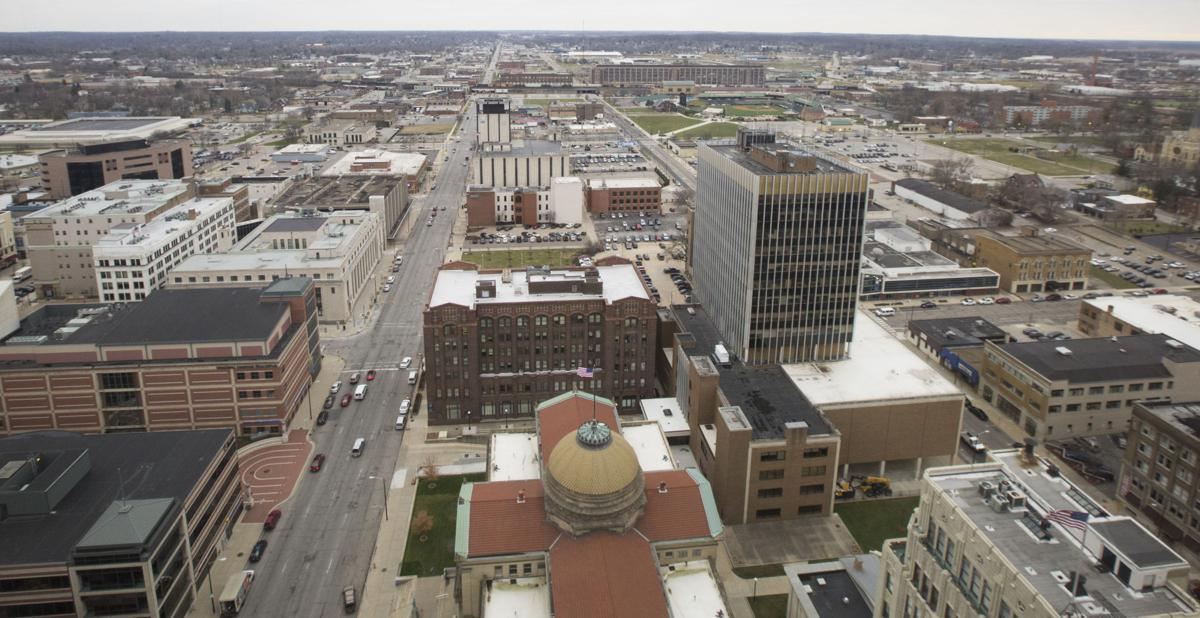
\includegraphics[scale=0.1]{south_bend}
\tiny{Photo:  Greg Swiercz, South Bend Tribune}   
\end{frame}



\begin{frame}{Project Goals}
\begin{center}
\textbf{Three main goals within this project}
\end{center}
\begin{enumerate}
    \item Conduct statistical tests and analysis of historical call center data using Python
     \item Utilize Python to create an open-source, accessible interactive dashboard of call center metrics
     \item Create a model and simulation of the call center, using statistical findings as basis
\end{enumerate}
\end{frame}


%----------------------------------------------------------------------------------------
%	Data
%----------------------------------------------------------------------------------------

\section{Data}

\begin{frame}{Data}
Publicly Available Data: 3 Main Sources
\begin{itemize}
    \item Daily Summary: 638 records
    \item Case Data: 488,601 records
    \item Topic Data: 99,516 records
\end{itemize}
Cleaning
\begin{itemize}
    \item Columns with open comment formats and many missing values dropped
    \item Other missing values imputed
    \item Attributes were created, such as duration and weekday attributes, from existing data
\end{itemize}
\end{frame}



%----------------------------------------------------------------------------------------
%	Analysis
%----------------------------------------------------------------------------------------


\section{Statistical Analysis} 


\begin{frame}{Call Volume}
	\begin{center}
		Calls by Month
	\end{center}
    \includegraphics[scale=0.3]{heatmap}
    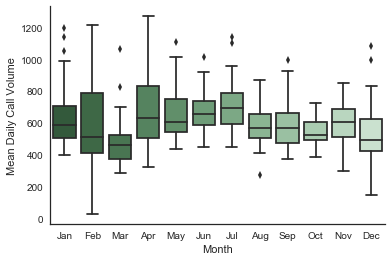
\includegraphics[scale=0.3]{monthly_boxplot}
    \begin{center}
    	Calls by Day
    \end{center}
    \includegraphics[scale=0.3]{daily_heatmap}
    \includegraphics[scale=0.3]{daily_call_boxplot}
\end{frame}
 


\begin{frame}{Other Statistical Analyses}
    \begin{itemize}
        \item Call duration by topic
        \item Call duration by department
        \item Call abandonment rates
        \item Hourly call volume means (for simulation)
\end{itemize}

\end{frame}




    
\section{Visualization}


\begin{frame}{Creating Visualization}
   \textbf{Goal: }Utilize Python to create an open-source, accessible interactive dashboard of call center metrics
\begin{itemize}
	\item Bokeh
	\begin{itemize}
		\item Open source package in Python
		\item HTML output:  Accessible, light, and easily hosted on web
	\item Utilizes JavaScript to create interactive visualizations
		\item Allows for more interaction and usefulness as opposed to static charts
		\end{itemize}
\end{itemize}
    
    
    
\end{frame}




\begin{frame}{Visualization Dashboard}
\begin{tabular}{cl}  
	\begin{tabular}{c}

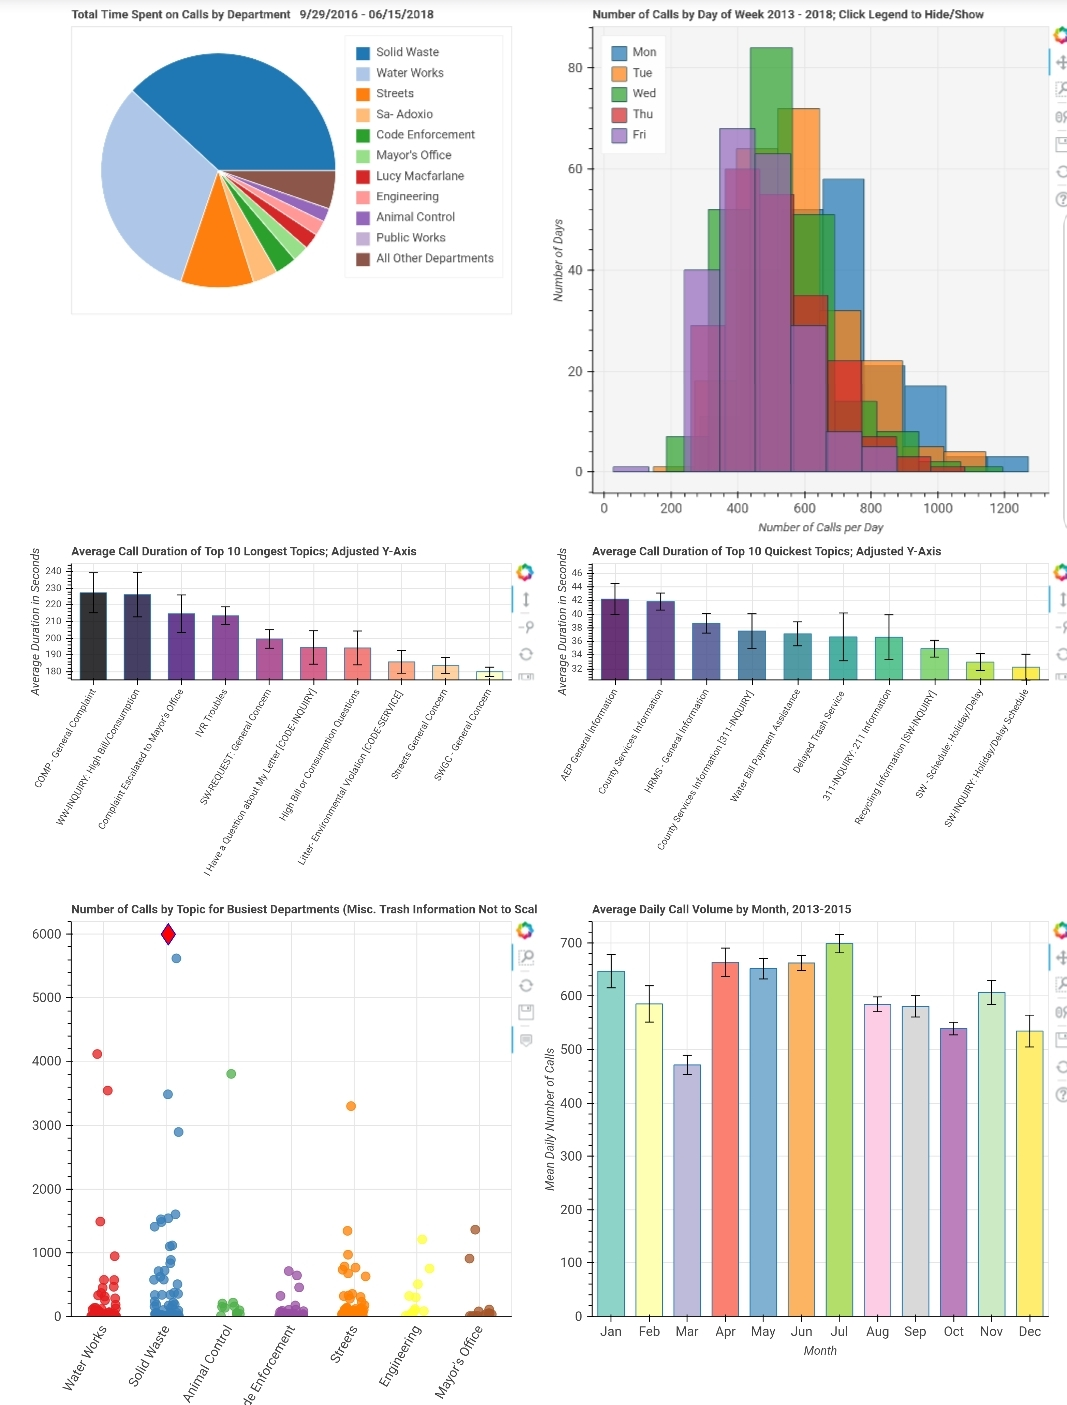
\includegraphics[scale=.15]{Dashboard}
	\end{tabular}
& \begin{tabular}{l}
\parbox{0.5\linewidth}{%  change the parbox width as appropiate
	\href{https://jdbul33.github.io/CallCenterDashboard.html}{Link to Hosted File}
}
\end{tabular}  \\
\end{tabular}


\end{frame}


\section{Simulation}

\begin{frame}{Simulation Summary}
\begin{itemize}
	\item \textbf{Goal: }Simulate the South Bend 311 Call Center as closely as possible given prior data
	\item Utilized Arena as simulation tool
	\item Historical distributions from prior analysis
	\begin{itemize}
		\item Topic, Duration, Call Volume
	\end{itemize}
	\item Explored operator staffing levels and scheduling
		\begin{itemize}
			\item Appeared to be close to optimally staffed
			\item Need operator metric data to compare for accuracy
		\end{itemize}
\end{itemize}

\end{frame}




\section{Conclusions}

\begin{frame}{Conclusions \& Wrap-Up}

All goals were met, with visualization dashboard hosted online and provided to the city.
\begin{itemize}
	\item Statistical tests and analysis were utilized in both visual identification/creation and model/simulation
	\item Interactive HTML dashboard created using Python showcasing metrics of interest to call center management
	\item Model of call center was created and simulations were run, replicating the actual operation as closely as possible
\end{itemize}


\end{frame}


%final thank you slide
\begin{frame}

\begin{center}
	{\Huge Thank You!} \\ %\hspace{.2cm}
	\begin{figure}
		%\centering
		\begin{minipage}[t]{0.48\textwidth}
			\centering
			\begin{itemize}
				\item Dr. Karl Schmitt
				\begin{itemize}
					\item Director, Analytics \& Modeling, Valparaiso University
				\end{itemize}
				\item Danielle Fulmer
				\begin{itemize}
					\item Director of Business Analytics, City of South Bend, IN
				\end{itemize}
			\end{itemize} 
		\end{minipage}\hfill
		\begin{minipage}[t]{0.48\textwidth}
			\centering
			\begin{figure}
				
\includegraphics[scale = 0.25]{Valpo}
			\end{figure}
			
\includegraphics[scale = 0.15]{seal}
		\end{minipage}\hfill
	\end{figure}
\end{center}
\end{frame}




\begin{frame}{References}
    \begin{itemize}
    \scriptsize{
        \item Baraka, H., Baraka, H. \& El-Gamily, I. (2013). Assessing call centers’ success: A validation of the DeLone and Mclean model for information systems. \textit{Egyptian Informatics Journal, 14}, 99-108.
        
        \item Chen, R-R., Chiang, Y., Chong, P.P., Lin, Y-H. \& Chang, H-K. (2011). Rough set analysis on call center metrics. \textit{Applied Soft Computing, 11}, 3804-3811.
        
        \item Brown, L., Gans, N., Mandelbaum, A., Sakov, A., Shen, H., Zeltyn, S. \& Zhao, L. (2005).
        Statistical analysis of a telephone call center: a queueing-science perspective. \textit{Journal of the
        American Statistical Association, 100} (469), 36-50.
        
        \item Zhang, X., Hong, L. \& Zhang, J. (2014). Scaling and modeling of call center arrivals. \textit{In
        Proceedings of the 2014 Winter Simulation Conference (WSC '14)}. IEEE Press, Piscataway, NJ,
        USA, 476-485.
        
        \item Bapat, V. \& Pruitte, E.B. Jr. (1998). Using simulation in call centers. \textit{In Proceedings of the
        30th conference on Winter simulation (WSC '98)}, D. J. Medeiros, Edward F. Watson, John S.
        Carson, and Mani S. Manivannan (Eds.). IEEE Computer Society Press, Los Alamitos, CA,
        USA, 1395-1400.
        
        \item Saltzman, R. \& Mehrotra, V. (2007). Managing trade-offs in call center agent scheduling:
        methodology and case study. \textit{In Proceedings of the 2007 Summer Computer Simulation Conference (SCSC '07)}. Society for Computer Simulation International, San Diego, CA, USA, 643-651.
        
        }
    \end{itemize}
\end{frame}


\end{document}